\documentclass[	a4paper,
			11pt,
			oneside,
			parskip]{scrartcl}
\usepackage{package/ownstil}
\usepackage{package/owncmd}

\bibliography{lit/lit.bib}



\begin{document}
\setlength{\parindent}{0pt} 
\onehalfspacing

%--------------------------------------------
% Inhaltsverzeichnis
\pagenumbering{Roman}
\tableofcontents 
\clearpage
\pagenumbering{arabic}
%--------------------------------------------

\section{Rahmenbedingungen und Zielstellung}

Ziel des Projektes ist die Realisierung eines Smartcard-basierten Ticketsystems für öffentliche Verkehrsmittel. Am Beispiel eines U-Bahn-Verkehrsnetzes soll es möglich sein, die Tickets auf der Karte zu speichern und Tickets über die Smartcard zu bezahlen. Hierzu soll der Fahrgast in der Lage sein, über die integrierte Geldbörse oder mittels angesammelter Bonuspunkte zu bezahlen. Des Weiteren soll es möglich sein den Fahrgast auf seiner Fahrt zu kontrollieren. Wurde das Ticket bereits beim Einlass kontrolliert und bestätigt, bleibt das Risiko das die Karte entwendet wurde. Ein Kontrolleur kann so während der Fahrt die Person anhand ihrer hinterlegten Daten und einem Bild, welches möglichst Platzsparend gespeichert wird, identifizieren. Die Kommunikation soll abgesichert sein damit Dritte keinen unberechtigten Zugriff auf die Daten der Smartcard erhalten können.

\section{Entwicklungsumgebung}

Nachfolgend werden alle eingesetzten Hilfsmittel zur Erstellung der On- und OffCard Anwendungen aufgeführt und erklärt. Hauptrolle spielen hierbei JCIDE für die Entwicklung der OnCard Applets und Eclipse zur Erstellung der OffCard Anwendung auf Basis von JavaFX.

\subsection{E(fx)lipse}

Um die OffCard Anwendung mit JavaFx entwickeln zu können wurde \tsl{Eclipse Mars} verwendet. Da in der aktuellen Version noch keine Integration von JavaFX besteht, kann es mit Hilfe des Plugins e(fx)lipse um die nötige Funktionalität erweitert werden.\medskip

Die Vorzüge von JavaFX liegen unter anderem im modularen Aufbau der Benutzeroberfläche. Diese wird als FXML-Datei aufgebaut und ist somit gekapselt vom restlichen Programmcode. Zusätzlich
können die UI-Elemente über CSS-Dateien optisch angepasst werden. Auch hier bietet e(fx)clipse eine sehr attraktiven FXML und CSS-Editor, welcher eine Autovervollständigung von Attributen bietet. 

\subsection{Package SmartcardIO}

Das Package SmartcardIO definiert eine Java-API für die Kommunikation mit Smartcards. Es ermöglicht Java-Anwendungen die Interaktion mit den Applets einer Smartcard, um so z.\,B. Daten auf der Karte zu verwalten. Eine \textit{TerminalFactory} erkennt alle angeschlossen Terminals und stellt eine Verbindung zur Karte her.\medskip

Über die Klasse \textit{CommandAPDU} lässen sich die zu übermittelnden Daten festlegen, inklusiver aller erforderlichen Parameter (CLA, INS, ...). Das Senden des Befehls geschieht über die verbundene Karte und der Funktion \textit{getBasicChannel().transmit()}.\medskip

War das Senden erfolgreich, erhält man die \textit{ResponseAPDU} und kann die Daten über \textit{getData()} und den Returncode über \textit{getSW()} auswerten.

\subsection{JCIDE}

JCIDE ist eine Entwicklungsumgebung die speziell für die Programmierung von JavaCards entwickelt wurde. Das Entwicklungskit erlaubt es schnell und einfach Applets mit den integrierten Tools zu erstellen. Der Grund für die Verwendung der IDE liegt in der Bereitstellung eines virtuellen Kartenlesegerätes und einer virtuellen Smartcard. Mit dem Übersetzen und Ausführen des Quelltextes werden die CAP-Dateien in einer virtuellen Smartcard bereitgestellt. Der Simulator
ist dabei ausschließlich für die Dauer der Ausführung aktiv. Über das virtuelle Kartenlesegerät können alle PC/SC kompatiblen Anwendungen mit dem Smartcard-Simulator kommunizieren.\medskip

\begin{figure}[!htb]
	\centering
  	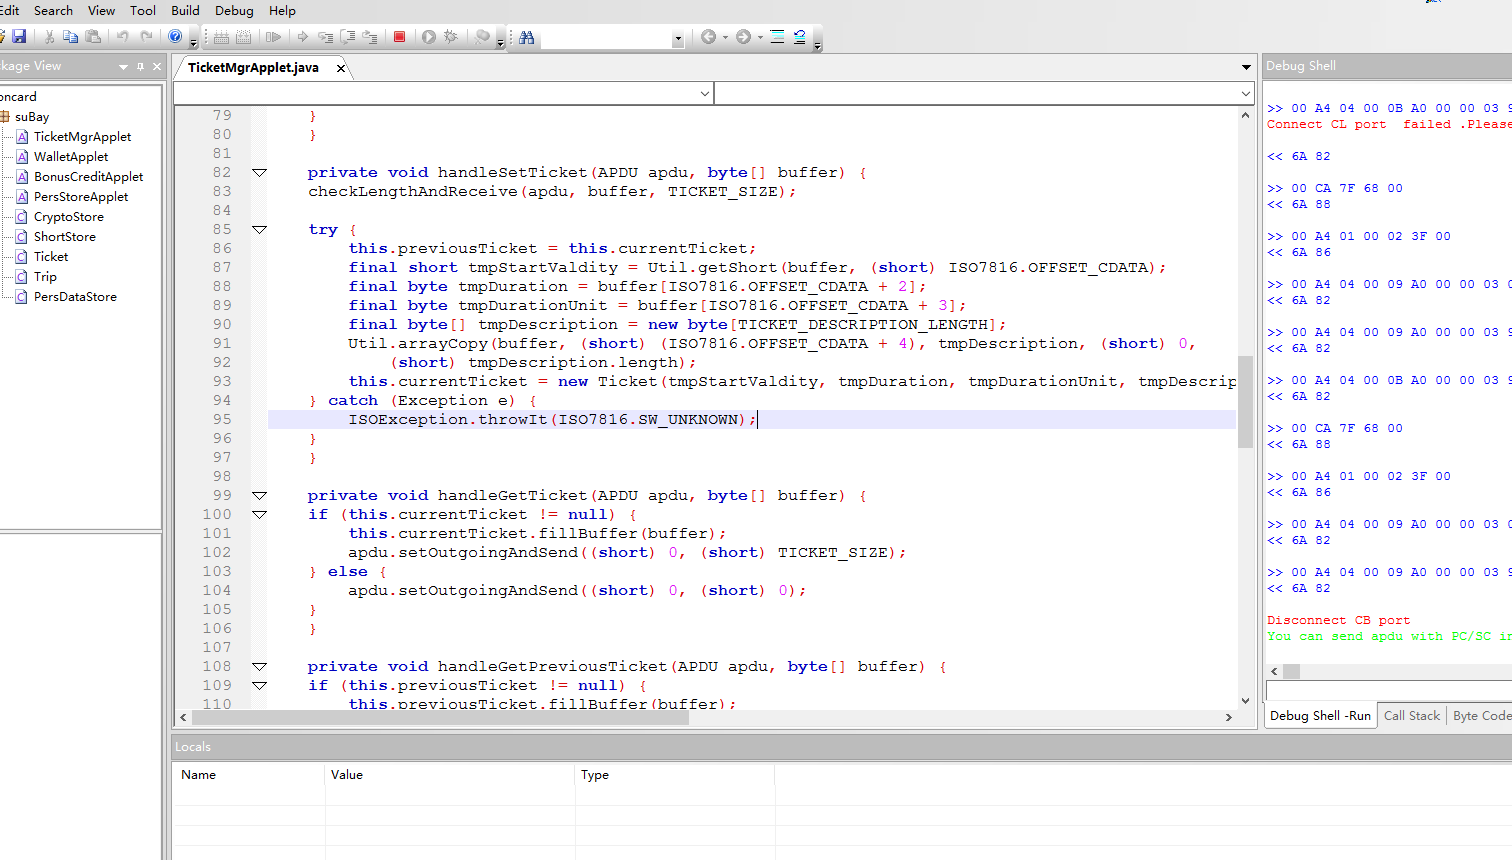
\includegraphics[width=0.95\textwidth]{img/jcide}
	\caption{JCIDE mit geöffneter Shell}
	\label{jcide}
\end{figure}

JCIDE wird von JAVACOS Technologies\footnote{\url{http://www.javacos.com/developmentkit.php}} entwickelt. Allerdings ist die Installation ausschließlich Windows-Systemen vorbehalten. \medskip

Weitere Vorteile bietet der integrierte Debugger, mit dem es möglich ist an jeder beliebigen Stelle Breakpoints zu setzen und somit schrittweise die Belegung aller Variablen zu zeigen.
Das Ausführen von Befehlen über die Debug-Shell ist ebenfalls möglich und ähnelt der Ausführung in Eclipse mit JCOP-Plugin. \medskip

Ein zusätzliches Tool (ebenfalls im Paket enthalten) ermöglicht die vereinfachte Kommunikation mit der Karte. Das als \glqq PyApduTool\grqq\/ bezeichnete Programm lädt die CAP-Datei aus dem Projektorder und zeigt alle gefundenen AID's auf. Somit entfällt die Eingabe des select-Befehls. Weiterhin existiert eine Ansicht, welche den send-Befehl übersichtlich aufteilt. Für jedes Byte existiert ein eigenes Eingabefeld. Diese Hilfe beugt Fehleingaben vor und speichert zusätzlich alle getätigten Operationen.

\subsection{SceneBuilder}

Der SceneBuilder unterstützt das Erstellen der FXML-Dateien zum Aufbau der Benutzeroberfläche. Alle unterstützen JavaFX UI-Elemente sind integriert und lassen sich per \glqq Drag and Drop\grqq\/ zur Bearbeitung in das eigene Programm-UI einfügen. Die Darstellung wird permanent aktualisiert. Somit ist jederzeit die konkrete Benutzeroberfläche ersichtlich. Ferner lassen sich alle Attribute zum ausrichten und beeinflussen der einzelnen Elemente direkt im Editor bearbeiten. Das Hinzufügen von IDs erleichtert zusätzlich den späteren Zugriff im Programmcode. Annotations (@FXML) an den jeweiligen Variablen schaffen die benötigte Verbindung.

\begin{figure}[!htb]
	\centering
  	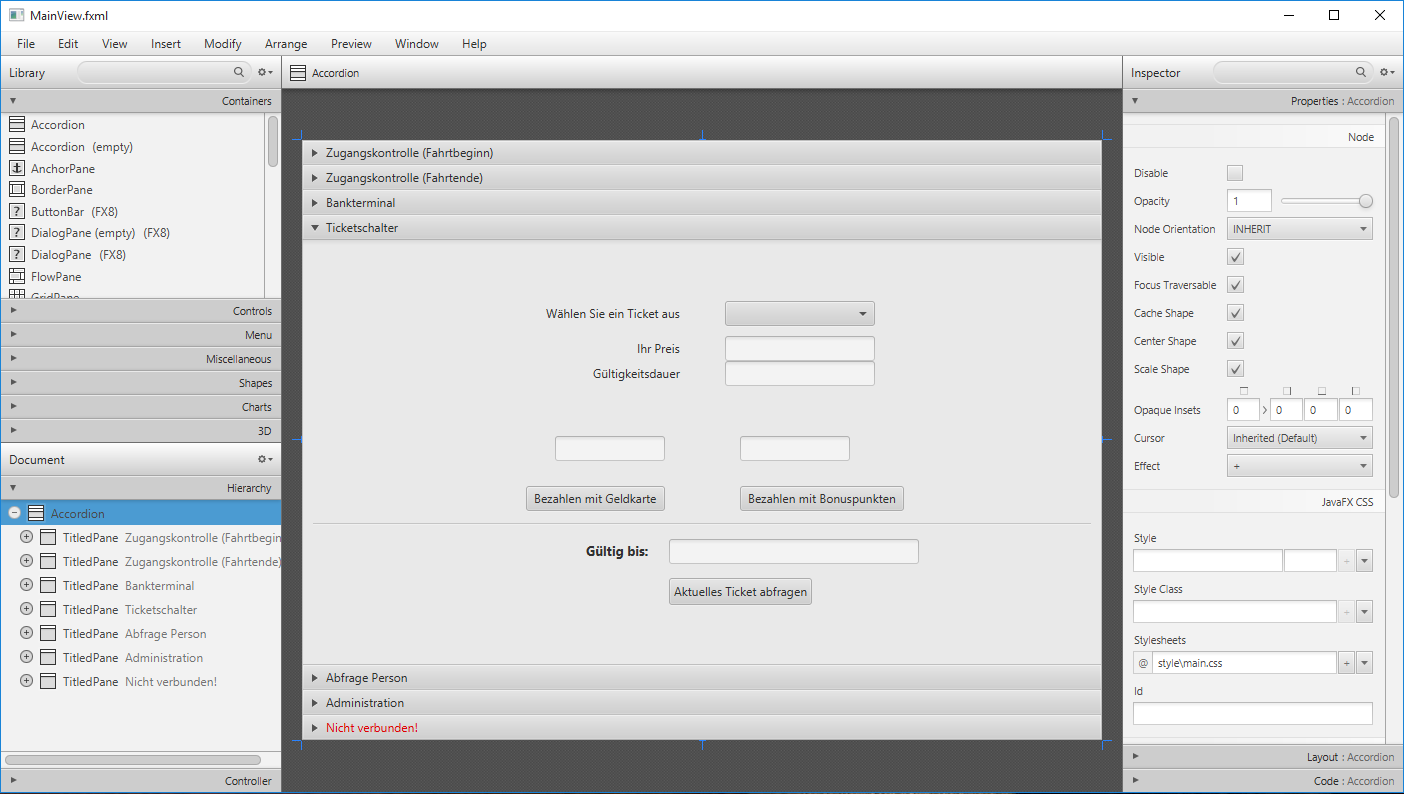
\includegraphics[width=0.95\textwidth]{img/scenebuilder}
	\caption{SceneBuilder}
	\label{scene}
\end{figure}

\subsection{GitHub}

Github stellt eine Hosting-Plattform für Softwareprojekte dar und kann einerseits kostenlos für Open Source-Projekte oder kommerziell für jegliche Art von Projekten eingesetzt werden. Die Verwaltung der Projekt-Repositorys erfolgt dabei über das dezentral organisierte Versionsverwaltungssystem \tsl{Git}, welches ursprünglich für die Entwicklung des Linux-Kernels von Linus Torvalds entwickelt wurde.

Alle relevanten Projekt-Bestandteile sind öffentlich in dem Projekt-Repository der Autoren auf GitHub\footnote{\url{https://github.com/philippsied/smartcard-course}} zu finden. Dies beeinhaltet neben den On- und OffCard Anwendungen ebenfalls diese Dokumentation. Somit ist das Projekt für jedermann zugänglich.

\section{Programmcode}

In diesem Abschnitt geht es um die Erläuterung der einzelnen Bestandteile des Projektes. Unterteilt in einen Architektur- und Implementierungsteil, werden die Aufgaben und Funktionsweisen der On- und OffCard Bestandteile einschließlich der dabei erstellten Schnittstellen erläutert. 

\subsection{Projektaufbau/Architektur}
 Der generelle Aufbau jeder Funktionalität folgt einem einheitlichen Schema. So besitzt jedes Applet (OnCard) seinen definierten Aufgabenbereich, weshalb insgesamt fünf Applets realisiert wurden: Für die Verwaltung der Geldbörse, der Bonuspunkte, der Fahrten, der Personaldaten und der kryptografischen Informationen bzw. Absicherung der Karte.
Dabei erfolgte der Aufbau der AIDs anhand folgendem Schemas:
   
\begin{table}[!htb]
  \centering
    \begin{tabular}{rl}
    \toprule
    \textbf{RID} & FD 75 42 61 79 (\glqq $^2$uBay\grqq) \\
    \textbf{PIX} & Individuell \\
    \midrule
    \textbf{AID} & RID + PIX \\
    \bottomrule
    \end{tabular}%
	\caption{Aufbau AID}
	\label{tab:strucaid}%
\end{table}%

Das obere Nibble des ersten Bytes der RID (0xF*) dient zur Kenntlichmachung, dass es sich um eine unregistrierte RID handelt.

Für die Kommunikation mit den OnCard-Bestandteilen wurden sämtliche OnCard-Instruktionen, einschließlich Konstanten für Fehlercodes und Puffergrößen, als Java-Interfaces\footnote{\glqq /OffCardAPP/src/main/java/clientAPI/impl/OncardAPI/\grqq} bereitgestellt. Auf Grundlage der OnCard-Interfaces wurden Schnittstellen für das 
UI erstellt\footnote{\glqq /OffCardAPP/src/main/java/clientAPI/\grqq} und diese für jedes Applet separat implementiert\footnote{\glqq /OffCardAPP/src/main/java/clientAPI/impl/\grqq}, wobei hier die eigentliche Kommunikation mit der Smartcard erfolgt. Das UI teilt sich durch die Verwendung von FXML nochmals in die Controller-Klassen\footnote{\glqq /OffCardAPP/src/main/java/controller/\grqq} und die FXML- sowie CSS-Dateien für das
UI\footnote{\glqq /OffCardAPP/src/main/java/main/UI/\grqq} auf. So soll eine konsequente Kapselung der Bestandteile erreicht werden, wodurch die Entwicklung der Applets, der Implementierung der Kommunikation mit den
Applets, die Verknüpfung mit dem UI und dem Design des UI selbst weitgehend unabhängig voneinander erfolgen kann. Exemplarisch ist hier die erfolgreiche sowie weitgehend parallele Entwicklung der Ticket- und Fahrtenverwaltung zu nennen.

\subsection{Funktionalität}
Bei der Erstellung der Applets wurde im Vorfeld festgelegt, dass die auszuführende Aktion eines Kommandos ausschließlich über das INS-Byte der APDU gesteuert werden soll, weshalb das Klassenbyte CLA auf \tbf{0xE0} und die Parameter-Bytes P1, P2 jeweils auf \tbf{0x00} festgeschrieben sind. Das Klassenbyte soll wie in \cite{ISO7816.2015} festgelegt signalisieren, dass es sich um ein eigenes Kommunikations-Format handelt, was sich hier jedoch ausschließlich auf das INS-Byte bezieht. Bei der Wahl der Fehlercodes wurde zudem auf die Vermeidung von Doppelbelegungen und Überschneidungen mit der ISO7816 geachtet. Bedingt durch die Limitierung des Smartcard-Simulators der JCIDE konnten ausschließlich Klassen des Javacard 2.2.2 Standards verwendet werden.


\subsubsection{Kryptografische Absicherung}
Um die Karte bis zu einem gewissen Maß vor gefälschten Kommandos zu schützen wurde ein Authentifizierungsmechanismus implementiert, der ein Senden von Kommandos ohne zuvor erfolgte Authentifizierung unterbinden soll.
Der Ablauf folgt einem vereinfachten Challenge-Response-Protokoll \cite{Eckert.2013}, wobei das Terminal zunächst die Challenge (64 Byte) von der Smartcard anfordert, diese durch die Javacard erzeugt und an das Terminal
zurückgeliefert wird. Das Terminal verschlüsselt die Challenge mit seinem privaten RSA-Schlüssel (2048 Bit) und sendet das Ergebnis an die Javacard. Mit dem hinterlegten öffentlichen Schlüssel wird die Challenge entschlüsselt und verglichen. Bei Übereinstimmung werden alle Kommandos bis zum Reset der Verbindung entgegengenommen. Der öffentliche Schlüssel muss bei der einmaligen Initialisierung der Karte durch den Aussteller/Administrator festgeschrieben werden. Zusätzlich kann eine Identifikationsnummer (ID) auf der Karte gespeichert werden um z.B. ein Whitelisting oder Blacklisting von Karten vorzunehmen. 

\paragraph{OnCard}
Das CryptoMgr-Applet dient einerseits für das Terminal als Authentifizierungsendpunkt, andererseits für die anderen Applets als Ansprechpartner, um die Rechtmäßigkeit von Kommandos zu prüfen. Hierfür implementiert es das
eigens erstellte \tsl{CryptoMgr}-Interface was wiederum das \tsl{Shareable}-Interface von Javacard erweitert. Um die Übertragung der 2048 Bit RSA-Schlüssel innerhalb eines Kommandos zu ermöglichen, muss das \tsl{ExtendedLength}-Interface von Java implementiert werden. Dadurch können Daten bis zu einer Länge von 65536 Bytes übertragen werden. Für die Speicherung der Challenge sowie des Verbindungszustandes werden ein transientes Byte-Array bzw. Byte verwendet.

\begin{table}[!htb]
  \centering
    \begin{tabular}{cc|cc}
    \toprule
    \textbf{PIX} 		& \multicolumn{3}{c}{43 72 79 70 74 6f 4d 67 72 (\glqq CryptoMgr\grqq)} \\
    \midrule
    \textbf{Daten} 		& \tbf{Größe} 	& \tbf{Funktion} & \tbf{INS} \\
    \hline
    Initialisierungsflag	& boolean		& Initialisieren 	& 0xEE \\
    KartenID\_h 		& short 		& Karten-ID abfragen 	& 0x10 \\
    KartenID\_l 		& short 		& Publickey abfragen 	& 0x20 \\
    Terminal-PublicKey		& RSAPublicKey 		& Challenge erhalten 	& 0xA0 \\
    Verbindungszustand		& byte (transient) 	& Response senden	& 0xB0 \\
    Aktuelle Challenge		& 64 Byte (transient) 	& 	&  \\
    \bottomrule
    \end{tabular}%
	\caption{PIX und Funktionsübersicht - CryptoManager}
	\label{tab:cryptodata}%
\end{table}%

\paragraph{OffCard} Der Zugriff auf das CryptoMgr-Applet teilt sich in den administrativen Zugriff für das Setzen des öffentlichen Schlüssels sowie der Karten-Id und in den operativen Zugriff zur Authentifizierung der Verbindung mit dem Terminal. Während die Karten-Id frei wählbar ist, wird der öffentliche Schlüssel zur Vereinfachung aus einem Keystore (LocalKeyStore) geladen, welcher einen festkodierten RSA-Schlüssel hält. Um eine Verschlüsselung
ohne Herausgabe des Schlüssels zu ermöglichen wird eine Lambda-Funktion (Schnittstelle EncryptFunction) verwendet. Diese wird über \tsl{LocalKeyStore\#getEncryptionFunc} bereitgestellt.

\subsubsection{Geldbörse}

Über die Geldbörse kann die Bezahlung der Tickets erfolgen, weshalb diese vor dem Ticketsystem realisiert werden musste. Zu den Funktionen gehören das Aufladen, Abbuchen sowie das Abfragen des Kontostandes.

\paragraph{OnCard} Zum Speichern des Geldbetrages wurde ein short-Wert definiert. Somit ist es möglich maximal 65536 Cent zu speichern. Dieser Betrag reich für die Geldbörse vollkommen aus, da ein Verlust der Karte auch den Verlust des Geldbetrages bedeuten würde.

\begin{table}[!htb]
  \centering
    \begin{tabular}{cc|cc}
    \toprule
    \textbf{PIX} 		& \multicolumn{3}{c}{57 61 6C 6C 65 74 (\glqq Wallet\grqq)} \\
    \midrule
    \textbf{Daten} 		& \tbf{Größe} 	& \tbf{Funktion} 	& \tbf{INS} \\
    \hline
    Geldbetrag 			& short 	& Geld aufladen 	& 0x10 \\
				&  		& Geld abbuchen 	& 0x20 \\
				& 		& Geld prüfen 		& 0x30 \\
    \bottomrule
    \end{tabular}%
      \caption{PIX und Funktionsübersicht - Geldbörse}
	\label{tab:walletdata}%
\end{table}%

Bei dem Abbuchen eines Geldbetrages wird geprüft, ob der angeforderte Betrag mindestens dem aufgeladenen Guthabens entspricht. Bei einem zu hohen Geldbetrag wird die Aktion mit einer Exception (0x6A83) beendet. Auch das Überschreiten des maximalen Guthabens wird durch eine Exception (0x6A84) abgefangen.

\paragraph{OffCard} Die OffCard-Anwendung zum aufladen der Geldkarte fällt entsprechend der wenigen Funktionen des Applets sehr klein aus. Über eine ComboBox lässt sich ein entsprechender Betrag zum aufladen schnell auswählen und über die Schaltfläche \textit{Aufladen} zur Karte übertragen. 

\begin{figure}[H]
	\centering
  	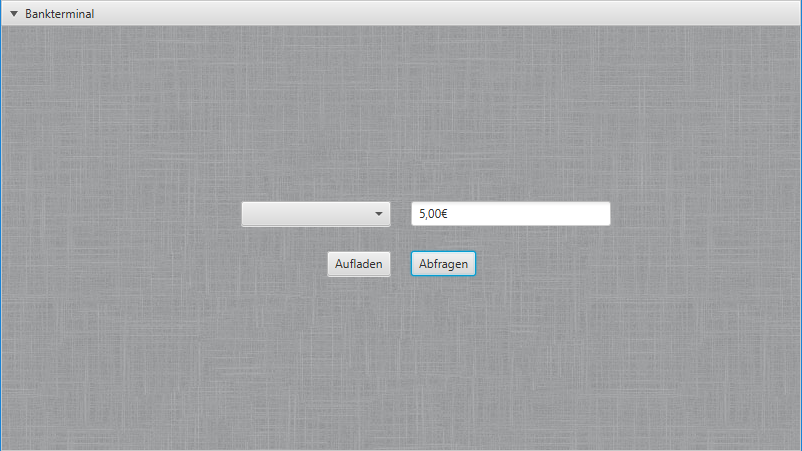
\includegraphics[width=0.95\textwidth]{img/wallet}
	\caption{Administration der Personendaten}
	\label{walletoff}
\end{figure}

Um den short-Wert in eine Byte-Folge zu konvertieren wurde mit der Klasse \textit{ByteBuffer} gearbeitet. Sie bietet die Möglichkeit beliebige Datentypen in eine Art Stapelspeicher abzulegen und als eine Byte-Folge bereitzustellen. Gleiches gilt für das entgegennehmen der Daten von der Karte. Die gelesenen Byte werden in den \textit{ByteBuffer} abgelegt und entsprechend der Datentypen herausgenommen. Hierbei ist auf die korrekte Reihenfolge der Informationen zu achten.

\subsubsection{Ticketsystem}

Das Ticketsystem ist fundamentale Grundlage für dieses Projekt. Nach der Implementierung der Geldkarte stehen der Entwicklung des Systems keine Hürden mehr im Wege. Des Weiteren soll durch die spätere Integration eines Bonussystems ein zweiter Zahlungsweg genutzt werden können. 

\paragraph{OnCard} Auf der Karte wird hierzu eine Beschreibung des Tickets sowie die nötigen Zeiten für den Gültigkeitszeitraum des Tickets gespeichert. Zum speichern einer Fahrt wird eine weitere Struktur benötigt. Diese hält alle Daten zum Antritt der Fahrt, wie den Zeitpunkt und den Namen der Station. Alle gespeicherten Zeiten werden bedingt durch ihre Größe (Unix-Zeitstempel) in zwei short-Variablen gespeichert. Die Aufteilung der int-Variable findet allerdings in der OffCard-Anwendung statt.


\begin{table}[!htb]
  \centering
    \begin{tabular}{cc|cc}
    \toprule
    \textbf{PIX} 	& \multicolumn{3}{c}{54 69 63 6b 65 74 4d 67 72 (\glqq TicketMgr\grqq)} \\
    \midrule
    \textbf{Daten} 	& \tbf{Größe} 	& \tbf{Funktion} 		& \tbf{INS} \\
    \hline
    \tbf{Ticket} 	&       	& Aktuelles Ticket setzen 	& 0x10 \\
    Beginn\_h 		& short 	& Aktuelles Ticket abfragen 	& 0x20 \\
    Beginn\_l 		& short 	& Vorheriges Ticket abfragen 	& 0x40 \\
    Ende\_h 		& short 	&       			&  \\
    Ende\_l 		& short  	&       			&  \\
    Beschreibung 	& 30 Byte  	&       			&  \\
    \hline
    \textbf{Fahrt} 	&   		& Fahr - Startzeit setzen 	& 0xA0 \\
    Beginn\_h 		& short 	& Fahrt - Endzeit setzen 	& 0xB0 \\
    Beginn\_l 		& short 	& Aktuelle Fahrt anzeigen 	& 0xC0 \\
    Station 		& 30 Byte 	&       			&  \\
    \bottomrule
    \end{tabular}%
      \caption{PIX und Funktionsübersicht - Ticketsystem}
	\label{tab:ticketfunc}%
\end{table}%


\paragraph{OffCard} Die OffCard-Anwendung fällt bei diesem System größer aus. Wie in Abbildung \ref{ticketoff} zu sehen, wird anhand einer \textit{ComboBox} das gewünschte Ticket ausgewählt. Die restlichen Felder geben zahlreiche Informationen zum Ticket selbst, bzw. die Zahlungsmöglichkeiten mit dem jeweiligen vorhandenen Guthabens. Ist genügend Guthaben auf der Geldkarte vorhanden, so wird dem Fahrgast zugleich das neue Guthaben (nach dem Kauf) angezeigt. Gleiches gilt für die Bezahlung mit Bonuspunkten.

Bei Auswahl der Schaltfläche \textit{Bezahlen mit Geldkarte} wird zunächst auf das Applet der Geldkarte zugegriffen und der Kontostand kontrolliert. Reicht dieser aus, wird der entsprechende Geldbetrag abgehoben. War der Vorgang erfolgreich und die ResponseAPDU signalisiert dies, wird das Ticket generiert. Der Gültigkeitszeitraum und die Beschreibung des Tickets (Kurzstrecke, etc.) wird dann zur Karte als eine Einheit gesendet. Jederzeit kann der Fahrgast über die Schaltfläche \textit{Aktuelles Ticket abfragen} den Gültigkeitszeitraum der gekauften Fahrkarte abfragen.

\begin{figure}[H]
	\centering
  	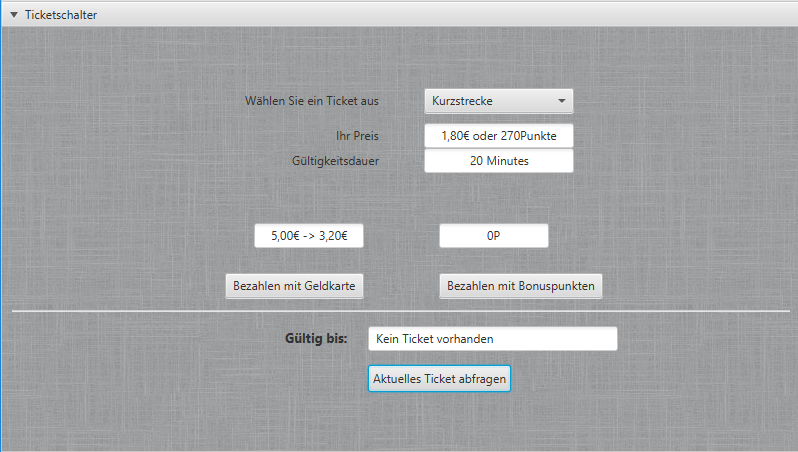
\includegraphics[width=0.95\textwidth]{img/ticket}
	\caption{Ticketschalter}
	\label{ticketoff}
\end{figure}

Zwei weitere OffCard-Anwendungen simulieren die Zugangskontrolle. Bei Fahrtantritt wird geprüft ob ein gültiges Ticket vorhanden ist. Ist dies der Fall, so wird eine Fahrt mit Zeitstempel des Fahrtantrittes und des Namen der Station auf der Smartcard gespeichert und die Schranke \glqq öffnet\grqq\ sich. Bei dem Beenden der Fahrt wird an der Ausgangskontrolle die Fahrtzeit geprüft und mit der Gültigkeitsdauer des Tickets verglichen.
Sofern das Ticket abgelaufen ist, werden die anfallenden Kosten bei einem simulierten Ticketserver abgefragt und das Geld von der Geldbörse abgezogen und es werden Bonuspunkte für die Fahrt gegeben. Sofern das Konto nicht ausreichend gedeckt ist wird der Auslass verweigert. Ein Kunde muss so zunächst sein Guthaben aufladen und erneut zur Ausgangskontrolle gehen.

\begin{figure}[H]
	\centering
  	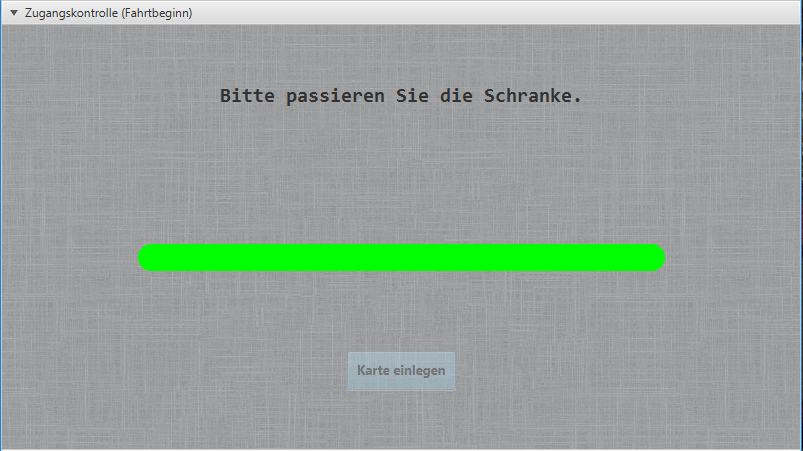
\includegraphics[width=0.95\textwidth]{img/gate}
	\caption{Zugangskontrolle}
	\label{gateoff}
\end{figure}

\subsubsection{Verwaltung der Personendaten}

Die Personendaten sollen der Kontrolle der Fahrgäste dienen. Hierzu werden die benötigten Daten im Vorfeld erhoben. Dazu zählen unter anderem der Name sowie das Geburtsdatum, aber auch ein Bild zur Identifikation soll gespeichert werden.

\paragraph{OnCard} Für die Speicherung der Daten auf der Karte wurde eine eigene Klasse erstellt, welche die erforderlichen Personeninformationen hält.

\begin{table}[!htb]
  \centering
    \begin{tabular}{cc|cc}
    \toprule
    \textbf{PIX} 	& \multicolumn{3}{c}{50 65 72 73 53 74 6F 72 65 (\glqq PersStore\grqq)} \\
    \midrule
    \tbf{Daten} 	& \tbf{Größe (Byte)} & \tbf{Funktion} & \tbf{INS} \\
    \hline
    Vorname 		& 10 Byte 		& Vornamen setzen 	& 0x1A \\
			&  		& Vornamen abfragen 	& 0x1B \\
    Nachname 		& 10 Byte  		& Nachnamen setzen 	& 0x2A \\
			& 		& Nachnamen abfragen 	& 0x2B \\
    Geburtsdatum 	& 10 Byte   		& Geburtsdatum setzen 	& 0x3A \\
			&  		& Geburtsdatum abfragen & 0x3B \\
    Wohnort 		& 15 Byte  		& Wohnort setzen 	& 0x4A \\
			&  		& Wohnort abfragen 	& 0x4B \\
    Straße 		& 25 Byte  		& Straße setzen 	& 0x5A \\
			&  		& Straße abfragen 	& 0x5B \\
    Telefonnummer 	& 15 Byte  		& Telefonnummer setzen 	& 0x6A \\
			&  		& Telefonnummer abfragen & 0x6B \\
    Bild  		& 6750 Byte  		& Bild setzen 		& 0x7A \\
			&       	& Bild abfragen 	& 0x7B \\
    \bottomrule
    \end{tabular}%
          \caption{PIX und Funktionsübersicht - Personaldaten}
  \label{tab:persdata}%
\end{table}%

In Tabelle \ref{tab:persdata} sind alle Funktionen zum Setzen und Lesen der Daten ersichtlich. Ferner lässt sich der reservierte Speicherplatz erkennen. Alle Informationen werden durch lesen des Buffers unter Nutzung der Funktion \textit{Util.arrayCopy()} entgegengenommen. Eine Übertragung einer längeren Zeichenfolge zur Karte ist möglich, wird aber bedingt durch den reservierten Speicherplatz abgeschnitten.

Schwieriger gestaltete sich die Übertragung des Bildes. Dieses kommt als 6750 Byte großes Array zur Karte. Da der Buffer nur 255 Byte entgegennimmt, muss mit der Funktion \textit{apdu.receiveBytes()} Bereichsweise das Bild in den Speicher geschrieben werden. Um die Übertragung der hohen Anzahl Bytes zu ermöglichen, wird der Sendevorgang im Extended-Mode initialisiert. Dies bedeutet, dass für das Feld LC (Länge des Datenbytes) nicht 1 Byte zur Verfügung steht, sondern 3 Byte. Zur Signalisierung der APDU wird das eigentliche Byte auf 0x00 gesetzt gefolgt von zwei weiteren Byte, welche die neue Länge des Datenfeldes repräsentieren.

\begin{center}
\begin{minipage}{0.9\textwidth} 
\begin{lstlisting}[language=Java]
// Aktuell gelesene Bytes
short read = apdu.setIncomingAndReceive();

// Gesamtlaenge
short footage = apdu.getIncomingLength();
	
// Ersten Bereich in Speicher schreiben - beginnend vom Offset		
personaldata.setPicPart(buf, (short)(ISO7816.OFFSET_EXT_CDATA), (short) 0, read);

// Zeiger im Speicher verschieben und restliche Bereiche schreiben		
while(read < footage) {
	short read_now = apdu.receiveBytes((short) 0);
	personaldata.setPicPart(buf, (short) 0, read, read_now);
	read += read_now;
}\end{lstlisting}
\end{minipage}
\end{center}

Das zurücksenden der Daten zur OffCard-Anwendung ist im Gegensatz stark vereinfacht. Sofern das Interface \textit{ExtendedLength} zum Applet hinzugefügt wurde, kann mit der Funktion \textit{apdu.sendBytesLong()} das komplette Bild (6750 Byte) gesendet werden.

\paragraph{OffCard} Das Problem der OffCard-Anwendung bestand in der Verkleinerung des Bildes für die Karte, da nur begrenzter Speicherplatz zur Verfügung steht. Für das Verkleinern des Bildes wurde die Klasse \textit{BufferedImage} verwendet. Hierzu kann nicht nur das Bild in Höhe und Weite verkleinert werden, sondern auch in ein Binärbild umgewandelt werden. Hierzu muss im Konstruktor der \textit{BufferedImage} der Parameter \textit{TYPE\_BYTE\_BINARY} angegeben werden. Die Konvertierung des Bildes erfolgt automatisch.

\begin{figure}[H]
	\centering
  	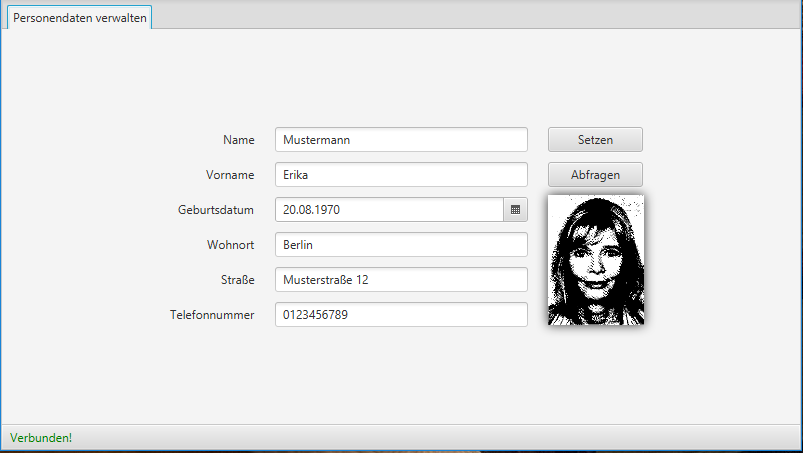
\includegraphics[width=0.95\textwidth]{img/pers}
	\caption{Administration der Personendaten}
	\label{pers}
\end{figure}

Nach dem Betätigen des Sende-Buttons werden alle Felder, sowie das Bild einzeln zur Karte gesendet. Gleiches gilt für die Abfrage der Daten.	
	
\subsubsection{Bonussystem}	

Das Bonussystem wurde als zweite Bezahlvariante eingeführt. Durch häufiges Fahren einer Strecke soll der Fahrgast mit Bonuspunkten belohnt werden.

\paragraph{OnCard} Das Bonussystem ist analog zur Geldkarte aufgebaut. Es finden beim Hinzufügen und Entfernen von Bonuspunkten die gleichen Prüfungen statt wie bei der Geldbörse. Sofern Fehler auftreten oder
die Prüfungen fehlschlagen, wird eine Exception an das Terminal gesendet.

\begin{table}[!htb]
  \centering
    \begin{tabular}{cc|cc}
    \toprule
    \textbf{PIX} 	& \multicolumn{3}{c}{42 6f 6e 75 73 43 72 65 64 69 74 (\glqq BonusCredit\grqq)} \\
    \midrule
    \textbf{Daten} 	& \tbf{Größe} 	& \tbf{Funktion} 	& \tbf{INS} \\
    \hline
    Bonuspunkte 	& short 	& Punkte aufladen 	& 0x10 \\
			&  		& Punkte abbuchen 	& 0x20 \\
			& 		& Punkte prüfen 	& 0x30 \\
    \bottomrule
    \end{tabular}%
              \caption{PIX und Funktionsübersicht - Bonussystem}
  \label{tab:bonusdata}%
\end{table}%

\paragraph{OffCard} Eine explizite OffCard-Anwendung existiert für den Zugriff auf das Bonussystem nicht. Einzig allein die Ausgangskontrolle schreibt die Bonuspunkte auf die Karte, sofern die Fahrt erfolgreich beendet wurde. Für jede gefahrene Minute werden 2 Punkte gutgeschrieben bis zu einem Maximalwert von 200 Punkten.
	
\section{Zusammenfassung \& Fazit}

Alle gesteckten Ziele konnten erreicht werden. Das Ticketsystem mit allen Bezahloptionen wurde realisiert und auch das verwerten der Tickets konnte simuliert werden. Gleiches gilt für den Erhalt von Bonuspunkten, die ohne der Simulation der Zugangskontrolle nicht möglich wären. Selbst die Speicherung der Personaldaten inklusive des Bildes konnte ohne Schwierigkeiten integriert werden.\medskip

Obwohl ursprünglich angedacht war, die kryptografische Absicherung mit Elliptische Kurven über endlichen Körpern ($F_p$) zu realisieren, musste die Implementierung verworfen werden, da sich deutliche Diskrepanzen bei der Spezifizierung der Kurven-Parameter des Javacard 2.2.2 Standards zeigten. Allgemein ist die jetztige Absicherung jedoch alles andere als praxistauglich, da ein Angreifer z.\,B. bereits durch ein MITM-Angriff die Kommandos zu seinen Gunsten verfälschen kann. Die Angriffsmöglichkeiten sind dabei weitaus vielfältig, weshalb ein Entwickler allein durch die kryptografische Absicherung voll ausgelastet wäre \cite{Markantonakis.2014}. Dennoch stellt das
eingesetzt Challenge-Response-Verfahren einen ersten und einfachen Schritt zur Absicherung dar.

Zu erwähnen sind die aufgetretenen Probleme im Zusammenhang mit der simulierten Smartcard. Nach mehrmaligen Austausch von APDUs beendete sich die Smartcard, d.\,h. die Ausführung in der JCIDE, ohne Angabe von Gründen. Der Fehler ist reproduzierbar tritt nach einer gewissen Anzahl an Befehlen auf.

Trotz der genannten Probleme und Hindernisse sehen die Autoren durch die funktionsfähige und umfangreiche Realisierung des Vorhabens eine erfolgreiche Umsetzung der Zielstellung, weshalb Sie das Projekt als Erfolg werten.

\clearpage
\printbibliography[heading=bibintoc]

\end{document}
